\section{例题与分析}

\begin{question}
\begin{example}[双缝前的不同滤光片]\label{ex:m21}
白光照射双缝，屏上原有彩色干涉条纹。现一缝前放只透红光的理想滤光片，另一缝前放只透绿光的理想滤光片。屏上会出现什么？
\begin{enumerate}[label=\Alph*.]
\item 只剩红色和绿色的双缝干涉条纹。
\item 红、绿双缝条纹消失，其余颜色条纹仍在。
\item 各色双缝干涉条纹均消失，但屏上仍有光。
\item 屏上完全黑暗。
\end{enumerate}
\end{example}
\fig{fig:m21q}{两缝各自只保留一种颜色，透射频带互不重叠}{
\begin{tikzpicture}
\draw[world] (0,-1.3)--(0,1.3);\draw[world] (5,-1.5)--(5,1.5);
\draw[ray] (-2,.6)--(0,.6);\draw[ray] (-2,-.6)--(0,-.6);
\node[left] at (-2,0) {白光};
\node[draw,fill=white,left] at (-.1,.6) {红滤片};
\node[draw,fill=white,left] at (-.1,-.6) {绿滤片};
\draw[ray] (0,.6)--(5,.5);\draw[ray] (0,-.6)--(5,.5);
\node[right] at (5,.5) {$P$};
\end{tikzpicture}}
\end{question}

\begin{solution}\textbf{对每种频率检查两缝是否都有振幅}\par\nobreak
图\ref{fig:m21q}中，红光只通过第一缝，绿光只通过第二缝。对任一频率而言，缺少另一缝中与它相干的同频分量，因此不能保留该频率的双缝条纹。

\fig{fig:m21s}{按频率分别追踪两路：每种颜色只有一路到达屏面}{\begin{tikzpicture}

\draw[world](0,-1.8)--(0,1.8);\draw[world](5,-1.8)--(5,1.8);
\fill[red](0,.8)circle(2pt);\fill[green!50!black](0,-.8)circle(2pt);
\node[left]at(0,.8){$S_1$：红};\node[left]at(0,-.8){$S_2$：绿};
\draw[ray,red](0,.8)--(5,.4);\draw[ray,green!50!black](0,-.8)--(5,.4);
\node[right]at(5,.4){$P$};
\node[align=center]at(2.5,2){红频率：$\mathcal E_{2r}=0$\quad 绿频率：$\mathcal E_{1g}=0$};
\node[align=center]at(2.5,-2.1){$I_r\propto|\mathcal E_{1r}|^2,\quad I_g\propto|\mathcal E_{2g}|^2$\\记录强度 $I(P)=I_r(P)+I_g(P)$};

\end{tikzpicture}}



\par\medskip\Needspace{4\baselineskip}\noindent\textbf{叠加到屏强度并判断选项}\par\nobreak
两束光仍能到达屏面，故选 \(\boxed{\mathrm C}\)。图\ref{fig:m21s}中的强度相加不要求光线完全不相遇；相遇也不自动产生可见干涉。每个有限宽单缝仍可有自身衍射包络，因此“无双缝条纹”不等于“屏上各处强度必然相同”。


\par\medskip\Needspace{4\baselineskip}\noindent\textbf{用观测时间检查红绿交叉项}\par\nobreak
从时间平均看，图\ref{fig:m21s}中红、绿两路虽在 $P$ 相遇，频率分量之间的交叉项含有 \(\cos[2\pi(\nu_{\text{红}}-\nu_{\text{绿}})t+\phi_0]\)，其变化远快于普通探测器的积分时间，平均贡献趋近于零。

理想滤片还使两缝没有共同透射频段；若实际滤片的频带有重叠，应单独检查重叠部分是否仍相干。
\end{solution}

\begin{question}
\begin{example}[固定路程差处的明暗]\label{ex:m22}
双缝到屏上 \(P\) 点的路程差为 \(\delta=0.6\,\mu\mathrm m\)。分别用频率
\(\nu_1=5.0\times10^{14}\,\mathrm{Hz}\)、
\(\nu_2=7.5\times10^{14}\,\mathrm{Hz}\) 的单色光照射双缝。判断两种情况下 \(P\) 为明纹还是暗纹。空气中取 \(c=3.0\times10^8\,\mathrm{m/s}\)。
\end{example}
\fig{fig:m22q}{\(P\) 点不动，改变的是波长与相位差}{
\begin{tikzpicture}
\coordinate (S1) at (0,.5);\coordinate (S2) at (0,-.5);\coordinate (P) at (5,1);
\draw[world] (0,-1)--(0,1);\draw[world] (5,-1)--(5,1.5);
\draw[ray] (S1)--(P);\draw[ray] (S2)--(P);
\node[left] at (S1) {$S_1$};\node[left] at (S2) {$S_2$};\node[right] at (P) {$P$};
\node at (2.5,-.8) {$r_2-r_1=0.6\,\mu\mathrm m$};
\end{tikzpicture}}
\end{question}

\begin{solution}\textbf{把两种频率换算成波长}\par\nobreak
图\ref{fig:m22q}的同一 $P$点具有固定路程差 $\delta$，明暗取决于它与波长之比。先求两种波长：
\[
 \lambda_1=\frac c{\nu_1}=0.60\,\mu\mathrm m,\qquad
 \lambda_2=\frac c{\nu_2}=0.40\,\mu\mathrm m.
\]


\par\medskip\Needspace{4\baselineskip}\noindent\textbf{以路程差除以各自波长}\par\nobreak
于是 \(\delta/\lambda_1=1\)，为明纹；\(\delta/\lambda_2=3/2\)，为暗纹。
\fig{fig:m22s}{等振幅复矢量相加：相差整周时同向，相差半周时反向}{\begin{tikzpicture}

\begin{scope}
\draw[axis,thick,blue](0,0)--(.9,0)node[midway,above]{$A_1$};
\draw[axis,thick,red](.9,0)--(1.8,0)node[midway,above]{$A_2$};
\draw[axis,very thick](0,-.65)--(1.8,-.65)node[midway,below]{$A_1+A_2$};
\node[below,align=center]at(.9,-1.35){$\Delta\phi_1=2\pi$\\同向叠加：明纹};
\end{scope}
\begin{scope}[xshift=5cm]
\draw[axis,line width=2pt,blue](0,0)--(1.8,0)node[midway,above]{$A_1$};
\draw[axis,thick,red,dashed](1.8,0)--(0,0)node[midway,below]{$-A_2$};
\node at(.9,-.85){合振幅为零};
\node[below,align=center]at(.9,-1.35){$\Delta\phi_2=3\pi$\\反向叠加：暗纹};
\end{scope}

\end{tikzpicture}}


\par\medskip\Needspace{4\baselineskip}\noindent\textbf{用复矢量核对相消条件}\par\nobreak
图\ref{fig:m22s}中，第二种光的传播相位差等效于 \(\pi\)，两缝等振幅时相消。所以结论是 $\nu_1$ 对应明纹、$\nu_2$ 对应暗纹。不要根据“频率越高越亮”判断某个固定点的明暗。
\end{solution}

\begin{question}
\begin{example}[第十级明纹的路程差]\label{ex:m23}
激光垂直照射双缝 \(S_1,S_2\)，波长为 \(\lambda\)。屏上 \(P\) 到两缝等距，记其明纹为零级。沿屏向上数，\(P_1\) 是第十级明纹。设 \(r_1=S_1P_1,r_2=S_2P_1\)，其中 \(S_1\) 为上缝。求 \(r_2-r_1\)。
\end{example}
\fig{fig:m23q}{先确定路程差的符号，再使用明纹级次}{
\begin{tikzpicture}
\draw[world] (0,-1)--(0,1);\draw[world] (5,-1)--(5,2);
\draw[axisline] (0,0)--(5,0);
\draw[ray] (0,.4)--(5,1.6) node[midway,above] {$r_1$};
\draw[ray] (0,-.4)--(5,1.6) node[midway,below] {$r_2$};
\node[left] at (0,.4) {$S_1$};\node[left] at (0,-.4) {$S_2$};
\node[right] at (5,0) {$P:\ k=0$};\node[right] at (5,1.6) {$P_1:\ k=10$};
\end{tikzpicture}}
\end{question}

\begin{solution}\textbf{根据屏上方位确定路程差正负}\par\nobreak
图\ref{fig:m23q}中，下缝到上方 \(P_1\) 的路程较长，故 \(r_2-r_1>0\)。

\par\medskip\Needspace{4\baselineskip}\noindent\textbf{将第十级代入相位条件}\par\nobreak
同相双缝的明纹条件是 \(r_2-r_1=k\lambda\)，因此
\[
 \boxed{r_2-r_1=10\lambda}.
\]
\fig{fig:m23s}{从零级走到十级，跨越十个同类条纹间隔}{
\begin{tikzpicture}[x=.65cm]
\draw[axis] (-.5,0)--(10.8,0) node[right] {$k$};
\foreach \x in {0,...,10}{\draw[thick] (\x,-.18)--(\x,.18);}
\node[below] at (0,-.18) {$P:0$};\node[below] at (10,-.18) {$P_1:10$};
\draw[dim] (0,.65)--(10,.65) node[midway,above] {$10\Delta x\ \longleftrightarrow\ 10\lambda$};
\end{tikzpicture}}


\par\medskip\Needspace{4\baselineskip}\noindent\textbf{区分级次和所数中心条数}\par\nobreak
图\ref{fig:m23s}中两个端点共有十一条明纹中心，间隔只有十个。明纹级次与“所数亮纹条数”应分清；明暗之间相差半级，但相邻两条明纹之间相差一级。
本题直接使用的是同相光源的相位条件，\(\delta=10\lambda\) 不需要先作小角近似。只有把级次换成屏上坐标 \(x_{10}\simeq10\lambda L/d\) 时，才需要远屏与小角条件。
\end{solution}

\begin{question}
\begin{example}[用劈尖条纹检查平整度]\label{ex:m24}
标准样板位于被检平面上方，左端接触，右端垫薄片，形成向右增厚的空气劈尖。反射光俯视图中，部分同级条纹在缺陷处向左弯曲。判断被检平面该处是凸起还是凹下。
\end{example}
\fig{fig:m24q}{空气膜向右增厚；图中竖线代表同级等厚条纹}{
\begin{tikzpicture}
\begin{scope}
\draw[world] (-1.7,0)--(1.7,0);
\draw[world] (-1.7,.1)--(1.7,.65);
\fill[pattern=north east lines] (1.45,0) rectangle (1.7,.61);
\node[below] at (0,0) {被检平面};
\node[above] at (0,.65) {标准样板};
\draw[axis] (-1.3,-.7)--(1.3,-.7) node[midway,below] {空气膜增厚};
\end{scope}
\begin{scope}[xshift=5cm]
\draw (-1.5,-1) rectangle (1.5,1);
\foreach \x in {-1.2,-.8,-.4,0,.4,.8,1.2}{
\draw[world] (\x,-1)--(\x,-.4) .. controls (\x-.4,-.2) and (\x-.4,.2) .. (\x,.4)--(\x,1);}
\node[below] at (0,-1.1) {条纹向左弯};
\end{scope}
\end{tikzpicture}}
\end{question}

\begin{solution}\textbf{按膜厚方向定义表面高度}\par\nobreak
按图\ref{fig:m24q}中膜向右增厚的方向，取右向为 \(x\) 正向，把被检面相对理想平面的高度记为 \(h(x,y)\)，凸起取 \(h>0\)。空气膜厚度为
\[
 t(x,y)=\alpha x-h(x,y).
\]


\par\medskip\Needspace{4\baselineskip}\noindent\textbf{追踪同一级等厚线的侧移}\par\nobreak
某一级条纹的厚度固定为 \(t_k\)，因此它的位置满足
\[
 x_k(y)=\frac{t_k+h(x_k,y)}{\alpha}.
\]
与无缺陷的位置 $x_{k0}=t_k/\alpha$ 相比，精确关系是 $\alpha\Delta x_k=h(x_k,y)$。若缺陷较小、侧移导致的 $h$ 变化可忽略，才进一步得到一阶侧移
\[
 \Delta x_k\simeq\frac h\alpha.
\]
\fig{fig:m24s}{固定同一膜厚：凹处应向薄端移动，凸处应向厚端移动}{\begin{tikzpicture}

\draw[axis](-4,0)--(4,0)node[right]{$x$};
\draw[world](0,-.6)--(0,.6) (-2.5,-.6)--(-2.5,.6);
\draw[aux](2.5,-.6)--(2.5,.6);
\draw[axis](0,1)--(-2.5,1)node[midway,above]{$h<0$};
\draw[axis](0,-1)--(2.5,-1)node[midway,below]{$h>0$};
\node[below]at(-2.5,-.6){凹处条纹};
\node[above]at(0,.6){理想条纹};
\node[above]at(2.5,.6){凸处条纹};

\end{tikzpicture}}


\par\medskip\Needspace{4\baselineskip}\noindent\textbf{结合左移方向判定凹凸}\par\nobreak
图\ref{fig:m24s}中，观察到左移意味着 \(\Delta x_k<0\)，从而 \(h<0\)，故缺陷为 \(\boxed{\text{凹下}}\)。物理上，凹处使空气膜变厚，要恢复同级条纹所需厚度，就必须移向较薄的左侧。这个解释也能检查代数符号。
\end{solution}

\begin{question}
\begin{example}[抽去一张垫片]\label{sup:m21}
两玻璃板形成空气劈尖，右端夹入两张等厚纸片。垫片到接触线的距离不变，现抽去一张，仍从上方观察同色单色光的反射条纹。条纹变疏、变密、不变还是消失？
\end{example}
\fig{fig:ms21q}{垫片数减半，几何长度保持不变}{
\begin{tikzpicture}
\draw[world] (-2,0)--(2,0);
\draw[world] (-2,.05)--(2,.65);
\fill[gray!25] (1.7,0) rectangle (2,.6);
\draw (1.7,.3)--(2,.3);
\node[right] at (2,.3) {两张};
\draw[aux] (-2,.05)--(2,.35);
\draw[dim] (-2,-.55)--(2,-.55) node[midway,below] {$\ell$};
\node[above] at (0,.7) {实线：原状态；虚线：抽去一张};
\end{tikzpicture}}
\end{question}

\begin{solution}\textbf{由垫片厚度反求两次劈角}\par\nobreak
设每张纸片厚 \(s\)，图\ref{fig:ms21q}的劈角先为
\(\alpha\simeq2s/\ell\)，抽去一张后 \(\alpha'\simeq s/\ell=\alpha/2\)。

\par\medskip\Needspace{4\baselineskip}\noindent\textbf{保持相邻级次的膜厚差不变}\par\nobreak
相邻同类条纹所需厚度差仍为 \(\lambda/2\)，故
\[
 \Delta x'=\frac{\lambda}{2\alpha'}=2\Delta x.
\]
\fig{fig:ms21s}{同一观察宽度内，条纹间距加倍}{
\begin{tikzpicture}
\foreach \x in {0,.4,...,4}{\draw[very thick] (\x,.3)--(\x,1);}
\foreach \x in {0,.8,...,4}{\draw[very thick] (\x,-1)--(\x,-.3);}
\node[left] at (0,.65) {两张};\node[left] at (0,-.65) {一张};
\draw[dim] (.8,-1.35)--(1.6,-1.35) node[midway,below] {$2\Delta x$};
\end{tikzpicture}}


\par\medskip\Needspace{4\baselineskip}\noindent\textbf{核对同一宽度内的条纹疏密}\par\nobreak
所以条纹 \(\boxed{\text{变疏}}\)。图\ref{fig:ms21s}中的间距增加源于相同厚度差对应更长水平距离；并非光的波长变大。
\end{solution}

\begin{question}
\begin{example}[四幅条纹与颜色]\label{ex:m25}
红光、蓝光分别通过同一双缝，黄光、紫光分别通过同一单缝，形成图\ref{fig:m25q}的四幅条纹。各实验的屏距相同，深色条表示亮纹。判断从左向右的颜色次序。
\end{example}
\fig{fig:m25q}{四幅候选图样使用相同图尺，深色条表示亮纹}{
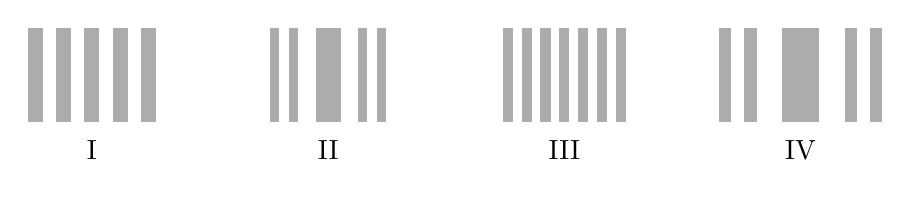
\begin{tikzpicture}[x=.8cm]
\begin{scope}
\foreach \x in {-.9,-.45,0,.45,.9}{\fill[gray!65] (\x-.12,0) rectangle (\x+.12,1.2);}
\node at (0,-.35) {I};
\end{scope}
\begin{scope}[xshift=3cm]
\fill[gray!65] (-.2,0) rectangle (.2,1.2);
\foreach \x in {-.85,-.55,.55,.85}{\fill[gray!65] (\x-.07,0) rectangle (\x+.07,1.2);}
\node at (0,-.35) {II};
\end{scope}
\begin{scope}[xshift=6cm]
\foreach \x in {-.9,-.6,-.3,0,.3,.6,.9}{\fill[gray!65] (\x-.08,0) rectangle (\x+.08,1.2);}
\node at (0,-.35) {III};
\end{scope}
\begin{scope}[xshift=9cm]
\fill[gray!65] (-.3,0) rectangle (.3,1.2);
\foreach \x in {-1.2,-.8,.8,1.2}{\fill[gray!65] (\x-.1,0) rectangle (\x+.1,1.2);}
\node at (0,-.35) {IV};
\end{scope}
\end{tikzpicture}}
\end{question}

\begin{solution}\textbf{按中央宽度和等间隔特征分类}\par\nobreak
先按形状分类：图\ref{fig:m25q}的 I、III 为双缝图样，II、IV 为单缝衍射图样。比较应在同一类内部进行，不能拿 I 的双缝间距直接与 II 的衍射中央宽度比较。

\fig{fig:m25s}{分别在同一类装置内比较波长与条纹尺度}{\begin{tikzpicture}[x=.65cm,y=.65cm]
\begin{scope}\draw[->](-3.2,0)--(3.3,0)node[right]{$x$};\draw[->](0,0)--(0,2.8)node[above]{$I$};
\draw[red,thick,domain=-3:3,samples=180]plot(\x,{2*cos(90*\x)^2});
\draw[blue,dashed,domain=-3:3,samples=180]plot(\x,{2*cos(135*\x)^2});
\node at(0,-.9){双缝：I（红）、III（蓝）};\end{scope}
\begin{scope}[xshift=5.2cm]\draw[->](-3.2,0)--(3.3,0)node[right]{$x$};\draw[->](0,0)--(0,2.8)node[above]{$I$};
\draw[orange!80!black,thick,domain=-3:3,samples=180]plot(\x,{2*(sin(90*\x)/(1.570796*(\x+.00001)))^2});
\draw[violet,dashed,domain=-3:3,samples=180]plot(\x,{2*(sin(135*\x)/(2.356194*(\x+.00001)))^2});
\node at(0,-.9){单缝：IV（黄）、II（紫）};\end{scope}
\end{tikzpicture}}


\par\medskip\Needspace{4\baselineskip}\noindent\textbf{在相同装置内比较波长}\par\nobreak
同一双缝的 \(d,L\) 相同，红光波长较长，所以 I 为红、III 为蓝。同一单缝的 \(a,L\) 相同，黄光波长长于紫光，所以 IV 为黄、II 为紫。由图\ref{fig:m25s}得次序
\[
 \boxed{\text{红、紫、蓝、黄}}.
\]


\par\medskip\Needspace{4\baselineskip}\noindent\textbf{用灰度图复核判别依据}\par\nobreak
彩色不是判别所必需的信息，单看规范画出的灰度条纹也可由宽度关系推断。
\end{solution}

\begin{question}
\begin{example}[单缝图样的辨认]\label{sup:m22}
单色光通过一条窄缝，在远处屏上形成衍射图样。图\ref{fig:ms22q}的四幅候选图中，亮纹画成深色，哪幅符合单缝衍射的基本特征？
\end{example}
\fig{fig:ms22q}{四幅候选图样，深色条表示亮纹}{
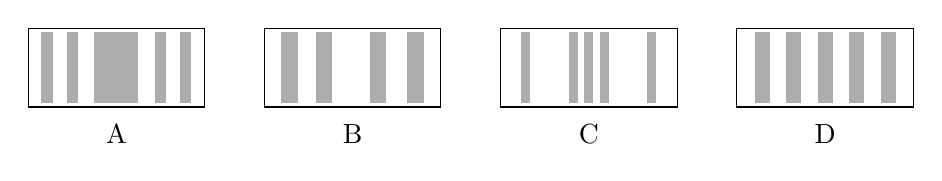
\begin{tikzpicture}[x=.8cm]
\foreach \z/\lab in {0/A,3/B,6/C,9/D}{
\begin{scope}[xshift=\z cm]
\draw (-1.4,0) rectangle (1.4,1);
\node at (0,-.35) {\lab};
\end{scope}}
\fill[gray!65] (-.35,.05) rectangle (.35,.95);
\foreach \x in {-1.1,-.7,.7,1.1}{\fill[gray!65] (\x-.09,.05) rectangle (\x+.09,.95);}
\begin{scope}[xshift=3cm]
\foreach \x in {-1,-.45,.4,1}{\fill[gray!65] (\x-.13,.05) rectangle (\x+.13,.95);}
\end{scope}
\begin{scope}[xshift=6cm]
\foreach \x in {-1,-.25,0,.25,1}{\fill[gray!65] (\x-.07,.05) rectangle (\x+.07,.95);}
\end{scope}
\begin{scope}[xshift=9cm]
\foreach \x in {-1,-.5,0,.5,1}{\fill[gray!65] (\x-.12,.05) rectangle (\x+.12,.95);}
\end{scope}
\end{tikzpicture}}
\end{question}

\begin{solution}\textbf{检查中央主峰和图样对称性}\par\nobreak
图\ref{fig:ms22q}中 A 的中央亮纹最宽，图样关于中心对称。B 缺少相应对称性，C 中心最窄，D 所有亮纹宽度相近，均不符合给定单缝的远场图样。故选 \(\boxed{\mathrm A}\)。

\fig{fig:ms22s}{第一暗纹确定中央亮纹的边界}{
\begin{tikzpicture}[x=1.2cm]
\draw[axis] (-2.8,0)--(2.8,0) node[right] {$x$};
\fill[gray!20] (-1,0) rectangle (1,1);
\draw[world] (-1,0)--(-1,1);\draw[world] (1,0)--(1,1);
\node[below] at (-1,0) {$-\lambda L/a$};
\node[below] at (1,0) {$+\lambda L/a$};
\draw[dim] (-1,1.3)--(1,1.3) node[midway,above] {$w_0=2\lambda L/a$};
\end{tikzpicture}}



\par\medskip\Needspace{4\baselineskip}\noindent\textbf{标出第一暗纹作为中央边界}\par\nobreak
图\ref{fig:ms22s}中的两条边界是第一暗纹。中央区宽度是它们之间的距离，而不是中心到单侧暗纹的距离。



\par\medskip\Needspace{4\baselineskip}\noindent\textbf{从缝内配对相消推导宽度}\par\nobreak
这项图样判据可由缝内连续波源相消得到：缝宽为 \(a\)，当 \(a\sin\theta=\lambda\) 时，把缝分成上下两半，相隔 \(a/2\) 的对应点相位相差 \(\pi\)，振幅逐对抵消。因此第一暗纹满足 \(\sin\theta=\pm\lambda/a\)，近轴屏坐标为 \(x_{\pm1}\simeq\pm\lambda L/a\)。相邻高阶暗纹间距约为 \(\lambda L/a\)，中央区却跨越正负第一暗纹，宽度为其两倍。这个定量关系支持图\ref{fig:ms22s}的选图结论，而非只凭“中心看起来较亮”判断。
\end{solution}

\begin{question}
\begin{example}[缝宽、缝距与条纹间距]\label{ex:m26}
用同一种单色光分别照射竖直单缝 \(a\) 和双缝 \(b\)，在远处屏上得到图样 \(c,d\)。判断：
\begin{enumerate}[label=\Alph*.]
\item \(c\) 为单缝衍射，\(d\) 为双缝干涉。
\item 单缝越宽，衍射展宽越明显。
\item 双缝间距越小，干涉条纹间距越大。
\item 照射双缝的波长越短，干涉条纹间距越大。
\end{enumerate}
\end{example}
\fig{fig:m26q}{缝板 \(a,b\) 与候选屏上图样 \(c,d\)；深色条表示亮纹}{
\begin{tikzpicture}
\draw[world] (0,-.8)--(0,-.12);\draw[world] (0,.12)--(0,.8);
\node[below] at (0,-1) {$a$};
\draw[world] (1.5,-.8)--(1.5,-.4);\draw[world] (1.5,-.2)--(1.5,.2);\draw[world] (1.5,.4)--(1.5,.8);
\node[below] at (1.5,-1) {$b$};
\foreach \x in {3,3.4,3.8,4.2,4.6}{\fill[gray!65] (\x,-.8) rectangle (\x+.14,.8);}
\node[below] at (3.8,-1) {$c$};
\fill[gray!65] (6.3,-.8) rectangle (6.9,.8);
\foreach \x in {5.6,5.95,7.2,7.55}{\fill[gray!65] (\x,-.8) rectangle (\x+.14,.8);}
\node[below] at (6.6,-1) {$d$};
\end{tikzpicture}}
\end{question}

\begin{solution}\textbf{先区分题图的两种条纹}\par\nobreak
图\ref{fig:m26q}中 \(c\) 是双缝干涉，\(d\) 是单缝衍射，A 颠倒。

\par\medskip\Needspace{4\baselineskip}\noindent\textbf{分别检查孔径和缝距的影响}\par\nobreak
单缝宽度增加时 \(2\lambda L/a\) 变小，衍射展宽减弱，B 错。由
\[
 \Delta x=\frac{\lambda L}{d}
\]
可知 C 对、D 错，故选 \(\boxed{\mathrm C}\)。
\fig{fig:m26s}{孔径宽度与双缝中心距在图中是两个不同的长度}{\begin{tikzpicture}[scale=.85]
\draw[thick](0,-1.6)--(0,-.35) (0,.35)--(0,1.6);\draw[<->](-.5,-.35)--(-.5,.35)node[left]{$a$};
\draw[->,blue](.2,0)--(2,0);\node[align=center]at(2.8,0){单缝中央宽度\\$2\lambda L/a$};
\draw[thick](5,-1.6)--(5,-.95) (5,-.65)--(5,.65) (5,.95)--(5,1.6);
\draw[dashed](4.5,-.8)--(5.2,-.8) (4.5,.8)--(5.2,.8);\draw[<->](4.5,-.8)--(4.5,.8)node[left]{$d$};
\draw[->,red](5.3,0)--(6.7,0);\node[align=center]at(7.8,0){细条纹间距\\$\lambda L/d$};
\node at(3.9,-2.3){每缝自身的宽度另控制衍射包络};\end{tikzpicture}}


\par\medskip\Needspace{4\baselineskip}\noindent\textbf{核对双缝自身宽度控制的包络}\par\nobreak
图\ref{fig:m26s}分别列出单缝宽度与双缝间距的影响。双缝中每条缝自身的宽度主要改变衍射包络，两缝中心间距主要决定细干涉条纹的间隔，计算时应使用各自对应的几何量。
\end{solution}

\begin{question}
\begin{example}[再辨干涉与衍射]\label{sup:m23}
单色光通过窄缝后形成图\ref{fig:ms23q}的甲、乙两幅图。判断哪幅为单缝衍射，哪幅为双缝干涉。两实验均使用 \(600\,\mathrm{nm}\) 的光，屏距均为 \(1.50\,\mathrm m\)，每条缝等宽。测得甲的中央亮纹宽 \(8.00\,\mathrm{mm}\)，乙的干涉细纹周期为 \(1.00\,\mathrm{mm}\)。求单缝宽度和双缝中心距，并判断乙的第几级干涉因子极大首先与单缝暗纹重合。
\end{example}
\fig{fig:ms23q}{甲、乙两次实验的屏上图样；深色表示亮纹，尺寸以测量值为准}{
\begin{tikzpicture}
\fill[gray!65] (-.3,0) rectangle (.3,1.2);
\foreach \x in {-1.2,-.8,.8,1.2}{\fill[gray!65] (\x-.1,0) rectangle (\x+.1,1.2);}
\node at (0,-.4) {甲};
\foreach \x in {3.6,4,4.4,4.8,5.2,5.6,6}{\fill[gray!65] (\x-.1,0) rectangle (\x+.1,1.2);}
\node at (4.8,-.4) {乙};
\end{tikzpicture}}
\end{question}

\begin{solution}\textbf{辨认甲乙并选取测量尺度}\par\nobreak
图\ref{fig:ms23q}中甲的中央亮纹显著宽于旁侧亮纹，乙具有细而近等间隔的条纹，故 \(\boxed{\text{甲为单缝衍射，乙为双缝干涉}}\)。几何示意图用来辨认特征，反求尺寸必须使用题给的测量数值，不能用尺量这幅示意图。
\fig{fig:ms23s}{归一化强度；横轴 \(q=a\sin\theta/\lambda\)，乙按题给数据取 \(d=4a\)}{
\begin{tikzpicture}[x=1.45cm,y=1.45cm]
\foreach \y/\t in {0/甲,-3.4/乙}{\begin{scope}[yshift=\y cm]
\draw[axis](-2.6,0)--(2.8,0)node[right]{$q$};
\draw[axis](0,0)--(0,1.2)node[above]{$I/I_{\max}$};
\node[left]at(-2.6,.8){\t};
\foreach \x in {-1,1}{\draw[aux](\x,0)--(\x,1);\node[below]at(\x,0){$\x$};}
\end{scope}}
\draw[thick,domain=-2.5:2.5,samples=400]plot(\x,{(sin(180*\x)/(pi*\x))^2});
\draw[dim](-1,-.35)--(1,-.35)node[midway,below]{中央宽度 $2$};
\begin{scope}[yshift=-3.4cm]
\draw[gray,dashed,domain=-2.5:2.5,samples=400]plot(\x,{(sin(180*\x)/(pi*\x))^2});
\draw[thick,domain=-2.5:2.5,samples=800]plot(\x,{(sin(180*\x)/(pi*\x))^2*cos(720*\x)^2});
\node[below,align=center]at(0,-.4){干涉因子周期 $\Delta q=a/d=0.25$};
\end{scope}
\end{tikzpicture}}

图\ref{fig:ms23s}直接比较两种强度分布：甲从 \(q=-1\) 到 \(q=1\) 为中央主峰；乙在同一包络内出现细纹。双缝条纹在更大范围内也会随单缝包络变弱，仅凭“边上变暗”不足以区分两类图样，还应检查中央宽度与细条纹周期。



\par\medskip\Needspace{4\baselineskip}\noindent\textbf{将细纹与单缝包络写成乘积}\par\nobreak
若每个狭缝宽 \(a\)、双缝中心距 \(d\)，两种模型在近轴远场分别给出
\[
 I_{\rm single}\propto\left(\frac{\sin\alpha}{\alpha}\right)^2,\qquad
 I_{\rm double}\propto\left(\frac{\sin\alpha}{\alpha}\right)^2
 \cos^2\!\left(\frac{\pi dx}{\lambda L}\right),\quad
 \alpha=\frac{\pi ax}{\lambda L}.
\]
图\ref{fig:ms23s}乙的细纹间距约为 \(\lambda L/d\)，外层包络仍由 \(a\) 控制。甲中央宽度为 \(2\lambda L/a\)，两侧相邻暗纹之间的宽度约为 \(\lambda L/a\)。辨认时应同时使用这些宽度关系和对称性；单独出现亮暗相间不足以确定缝数。


\par\medskip\Needspace{4\baselineskip}\noindent\textbf{反求缝宽和两缝中心距}\par\nobreak
由甲的中央两第一暗纹间距反求
\[
 a=\frac{2\lambda L}{w_0}
 =\frac{2(600\times10^{-9})(1.50)}{8.00\times10^{-3}}
 =\boxed{0.225\,\mathrm{mm}},\qquad
 d=\frac{\lambda L}{\Delta x}=\boxed{0.900\,\mathrm{mm}}.
\]
于是 \(d/a=4\)。



\par\medskip\Needspace{4\baselineskip}\noindent\textbf{联立两种条件判断首个缺级}\par\nobreak
图\ref{fig:ms23s}乙的第一包络零点在 \(q=\pm1\)，而第 \(k\) 级干涉因子极大在 \(q=ka/d=k/4\)，两者首先在 \(k=\pm4\) 重合。故首先缺失的是 \(\boxed{\text{第 }4\text{ 级}}\)。第4级的位置仍满足缝间相长条件，但每条缝单独向这个方向的振幅都为零，因而合成强度也为零；这正是把干涉与衍射同时考虑的必要性。
\end{solution}

\begin{question}
\begin{example}[立体电影的偏振配置]\label{ex:m27}
两台放映机分别投射左眼画面 \(L\) 和右眼画面 \(R\)，银幕保持偏振。表中“放映片”表示相应放映机偏振片的透振方向。哪种配置能使每只眼只接收自己的画面？竖、横表示互相垂直的两个方向。
\[
\begin{array}{c|cccc}
 &L\text{放映片}&\text{左镜片}&R\text{放映片}&\text{右镜片}\\\hline
 A&\text{竖}&\text{竖}&\text{竖}&\text{竖}\\
 B&\text{竖}&\text{竖}&\text{横}&\text{横}\\
 C&\text{竖}&\text{横}&\text{横}&\text{竖}\\
 D&\text{横}&\text{横}&\text{横}&\text{横}
\end{array}
\]
\end{example}
\fig{fig:m27q}{两路画面共用银幕，利用偏振方向选择接收通道}{
\begin{tikzpicture}
\node[draw] (L) at (0,1) {左眼画面 \(L\)};
\node[draw] (R) at (0,-1) {右眼画面 \(R\)};
\node[draw,minimum height=2.3cm] (S) at (3.3,0) {银幕};
\node[draw] (EL) at (6.7,1) {左眼};
\node[draw] (ER) at (6.7,-1) {右眼};
\draw[ray] (L)--(S);\draw[ray] (R)--(S);
\draw[ray] (S)--(EL);\draw[ray] (S)--(ER);
\end{tikzpicture}}
\end{question}

\begin{solution}\textbf{为每只眼写出保留和阻断条件}\par\nobreak
图\ref{fig:m27q}中两路画面共用银幕，应在眼镜处选择接收通道。对左眼画面，左镜片应与其偏振方向平行，右镜片应与其正交；右眼画面则相反。

\par\medskip\Needspace{4\baselineskip}\noindent\textbf{代入平行与正交的透过率}\par\nobreak
由马吕斯定律，平行通道 \(\cos^20=1\)，正交通道 \(\cos^290^\circ=0\)，所以选 \(\boxed{\mathrm B}\)。
\fig{fig:m27s}{B 配置的透过关系；对角通道通过，交叉通道阻断}{
\begin{tikzpicture}
\node[draw] (L) at (0,1) {\(L:\ \updownarrow\)};
\node[draw] (R) at (0,-1) {\(R:\ \leftrightarrow\)};
\node[draw] (EL) at (5,1) {左镜：\(\updownarrow\)};
\node[draw] (ER) at (5,-1) {右镜：\(\leftrightarrow\)};
\draw[axis] (L)--(EL) node[midway,above] {通过};
\draw[axis] (R)--(ER) node[midway,below] {通过};
\draw[aux] (L)--(ER);\draw[aux] (R)--(EL);
\node[fill=white] at (2.5,0) {交叉通道为零};
\end{tikzpicture}}


\par\medskip\Needspace{4\baselineskip}\noindent\textbf{检查四种配置的画面归属}\par\nobreak
图\ref{fig:m27s}中两条实线分别保留了左右视差信息。A、D 使两眼都收到相同的混合画面；C 把两路画面交换给了错误的眼睛。若银幕完全破坏偏振，上述选择机制就失效，不能仅靠眼镜恢复。
\end{solution}

\begin{question}
\begin{example}[旋光法测浓度]\label{ex:m28}
自然光源 \(S\) 后依次放起偏器 \(A\)、待测糖溶液 \(P\)、检偏器 \(B\)，最后在 \(O\) 观察。不放溶液时转动 \(B\)，使 \(O\) 处最亮；再插入使偏振方向转过 \(\alpha\) 的溶液，忽略吸收。
求强度如何改变，以及分别只转动 \(A\) 或只转动 \(B\) 时恢复最大亮度所需的角度。测浓度时固定波长、温度与溶液厚度。
\end{example}
\fig{fig:m28q}{光的传播次序为 \(S\to A\to P\to B\to O\)}{
\begin{tikzpicture}
\draw[axis] (-1,0)--(7.7,0);
\node[left] at (-1,0) {$S$};
\foreach \x/\lab in {0/A,3/P,6/B}{
\draw[world] (\x,0) ellipse(.3 and .85);\node[above] at (\x,.85) {\(\lab\)};}
\draw[very thick] (0,-.65)--(0,.65);
\draw[very thick] (6,-.65)--(6,.65);
\node[below] at (3,-1) {旋转 \(\alpha\)};
\node[right] at (7.7,0) {$O$};
\end{tikzpicture}}
\end{question}

\begin{solution}\textbf{沿元件次序计算插入后的强度}\par\nobreak
按图\ref{fig:m28q}的 $A\to P\to B$次序，把起偏器后的强度记为 \(I_p\)，初始 \(A,B\) 平行。不放溶液时 \(I_{\max}=I_p\)，插入后偏振方向相对 \(B\) 转过 \(\alpha\)，故
\[
 \boxed{I=I_{\max}\cos^2\alpha}.
\]
强度变化由偏振方向与检偏器透振轴的夹角决定；下面用实际导数判断微小旋光角的亮度灵敏度。
\fig{fig:m28s}{沿传播方向看横截面；虚线为 \(B\) 最初的透振方向}{
\begin{tikzpicture}
\draw[aux] (0,-1.2)--(0,1.2);
\draw[axis,thick] (0,0)--(0,1);
\node[above right] at (.12,1.15) {\(A,B\) 初始};
\draw[axis,thick] (0,0)--(-.65,.85);
\node[left] at (-.8,.65) {\(P\) 后偏振};
\draw[axis] (0,.65) arc(90:128:.65);
\node at (-.3,.36) {$\alpha$};
\node[draw,align=center] at (4,0)
{只转 \(B\)：沿旋光方向转 \(+\alpha\)\\只转 \(A\)：逆旋光方向转 \(-\alpha\)};
\end{tikzpicture}}


\par\medskip\Needspace{4\baselineskip}\noindent\textbf{分别求转动起偏器和检偏器的方向}\par\nobreak
按图\ref{fig:m28s}约定旋光方向为正。只转 \(B\) 时，使其与出射偏振方向平行，须转 \(+\alpha\)；只转 \(A\) 时，溶液仍额外转动 \(+\alpha\)，故应预先把入射偏振方向转 \(-\alpha\)。两个透振方向以 $180^\circ$ 为周期；最小转角应把 $+\alpha$ 或 $-\alpha$ 归约到 $[-90^\circ,90^\circ]$ 后取绝对值。通常小旋光角时，最小转角大小均为 $|\alpha|$。



\par\medskip\Needspace{4\baselineskip}\noindent\textbf{检查微小角的亮度灵敏度}\par\nobreak
固定 $I_p$，对 $I=I_p\cos^2\alpha$ 使用链式法则，
\[
 \frac{\dd I}{\dd\alpha}=2I_p\cos\alpha(-\sin\alpha)=-I_p\sin2\alpha,
 \qquad \frac{\dd^2I}{\dd\alpha^2}=-2I_p\cos2\alpha.
\]
在 $\alpha=0$，三项分别为 $I_p,0,-2I_p$；函数关于零点为偶函数，因此泰勒式给出 $I/I_p=1-\alpha^2+O(\alpha^4)$，角度须用弧度。最大亮度附近的变化是二阶量，微小转角造成的降低可能很小。在平行和正交位置，一阶导数均为零；其绝对值在约 $45^\circ$ 处最大。实际角度测量还应兼顾亮度噪声和所用检偏方法，不能把“接近消光”简单等同于斜率最大。



\par\medskip\Needspace{4\baselineskip}\noindent\textbf{在固定实验条件下反求浓度}\par\nobreak
测量时利用恢复最大强度或消光位置的角度，结合固定条件下的 \(\alpha=[\alpha]\ell c_s\) 求浓度。这样比较的是方向变化，可避免把吸收引起的强度降低全部误认为旋光。
\end{solution}

\begin{question}
\begin{example}[洛埃镜的干涉区域与条纹间距]\label{ex:m29}
点光源 \(S\) 位于水平镜面上方 \(a\)，屏在其右侧水平距离 \(L\) 处。镜面 \(M\) 只覆盖 \(x_1\le x\le x_2\)，其中 \(0<x_1<x_2<L\)。光源坐标为 \((0,a)\)，屏为 \(x=L\)。
画出直接光和反射光在屏上的重叠区域，并求近轴条件下相邻同类条纹的间距。设波长为 \(\lambda\)，镜面引入相对 \(\pi\) 反射相位。
\end{example}
\fig{fig:m29q}{有限长度镜面决定可接收反射光的屏上范围}{
\begin{tikzpicture}[x=.9cm]
\draw[axisline] (-.5,0)--(7,0);
\draw[world,line width=1.2pt] (1.5,0)--(4.5,0);
\draw[world] (6,-1.5)--(6,3);
\fill (0,1) circle(1.4pt) node[left] {$S(0,a)$};
\node[below] at (1.5,0) {$x_1$};\node[below] at (4.5,0) {$x_2$};
\node[right] at (6,2.7) {屏 \(x=L\)};
\node[above] at (3,0) {$M$};
\end{tikzpicture}}
\end{question}

\begin{solution}\textbf{用镜像光源构造有限镜面的照明区}\par\nobreak
将图\ref{fig:m29q}中的 \(S\) 关于镜面反射到 \(S'(0,-a)\)。镜面反射光等效于从 \(S'\) 发出、穿过实际镜面区间的光。图\ref{fig:m29s}中，连接 \(S'\) 与镜面两端并延长，得到屏上的 \(P_{\text{高}},P_{\text{低}}\)。直线从 \(S'\) 经 \((x_m,0)\) 到屏，交点高度为
\[
 y=a\left(\frac L{x_m}-1\right).
\]
所以反射光照到的区间为
\[
 \boxed{a\left(\frac L{x_2}-1\right)\le y
 \le a\left(\frac L{x_1}-1\right)}.
\]
若直接光可照满这段屏面，则此区间就是几何重叠区；实际还应满足两束光相干且均有可观测强度。
\fig{fig:m29s}{由虚光源和镜面端点构造重叠区；纵向作压缩示意}{
\begin{tikzpicture}[x=.9cm,y=.72cm]
\draw[axisline] (-.4,0)--(6.7,0);
\draw[world,line width=1.2pt] (1.5,0)--(4.5,0);
\draw[world] (6,-1.4)--(6,3.6);
\fill[gray!18] (5.85,.333) rectangle (6,3);
\coordinate (S) at (0,1);\coordinate (Sp) at (0,-1);
\draw[aux] (Sp)--(1.5,0);\draw[aux] (Sp)--(4.5,0);
\draw[ray] (S)--(1.5,0);\draw[ray] (1.5,0)--(6,3);
\draw[ray] (S)--(4.5,0);\draw[ray] (4.5,0)--(6,.333);
\draw[ray] (S)--(6,1.7);
\node[left] at (S) {$S$};\node[left] at (Sp) {$S'$};
\node[right] at (6,3) {$P_{\text{高}}$};\node[right] at (6,.333) {$P_{\text{低}}$};
\node[below] at (1.5,0) {$x_1$};\node[below] at (4.5,0) {$x_2$};
\end{tikzpicture}}



\par\medskip\Needspace{4\baselineskip}\noindent\textbf{由等效双光源求几何路程差}\par\nobreak
对于屏上任意点 \(P(L,y)\)，反射光路长等于 \(S'P\)。用两根式的平方差消去相减，几何路程差为
\begin{align*}
 \delta&=\sqrt{L^2+(y+a)^2}-\sqrt{L^2+(y-a)^2}\\
 &=\frac{(y+a)^2-(y-a)^2}
 {\sqrt{L^2+(y+a)^2}+\sqrt{L^2+(y-a)^2}}\\
 &=\frac{4ay}{\sqrt{L^2+(y+a)^2}+\sqrt{L^2+(y-a)^2}}
 \simeq\frac{2ay}{L}.
\end{align*}


\par\medskip\Needspace{4\baselineskip}\noindent\textbf{求相邻同类条纹的近轴间距}\par\nobreak
这里要求 \(a,|y|\ll L\)。由相邻同类条纹 \(\Delta\delta=\lambda\)，
\[
 \boxed{\Delta y=\frac{\lambda L}{2a}}.
\]
两等效光源间距为 \(2a\)，不能漏掉这个 2。



\par\medskip\Needspace{4\baselineskip}\noindent\textbf{加入反射相移并检查可见区域}\par\nobreak
反射还增加相对相位 \(\pi\)，故
\[
 \Delta\phi=\frac{2\pi\delta}{\lambda}+\pi.
\]
理想延拓到 \(y=0\) 时为暗纹，与同相双缝的中央明纹相反。但有限镜面的 \(P_{\text{低}}\) 通常高于 \(y=0\)，中央暗纹可能不在实际可见区。半波损失改变明暗级次位置，不改变相邻同类条纹间距。
\end{solution}

\begin{question}
\begin{example}[阈值、光强与初动能]\label{ex:m210}
对同一种金属，以下说法哪些正确？
\begin{enumerate}[label=\Alph*.]
\item 入射光频率低于阈值时，通常的一光子光电效应不能发生。
\item 无论频率多低，只要照射足够久就会发生光电效应。
\item 频率超过阈值时，光强越弱，光电子最大初动能越小。
\item 频率超过阈值时，频率越高，光电子最大初动能越大。
\end{enumerate}
\end{example}
\fig{fig:m210q}{分别考虑单个光子的能量与单位时间到达的光子数}{
\begin{tikzpicture}
\node[draw,align=center] at (0,0) {改变频率\\每个光子能量 \(h\nu\) 改变};
\node[draw,align=center] at (5,0) {固定频率、改变光强\\光子到达率改变};
\draw[axis] (0,-.7)--(2,-1.5);
\draw[axis] (5,-.7)--(3,-1.5);
\node[draw] at (2.5,-2) {同一金属，逸出功 \(W\) 固定};
\end{tikzpicture}}
\end{question}

\begin{solution}\textbf{用单次吸收的能量条件判断阈值}\par\nobreak
图\ref{fig:m210q}把单光子能量与光子到达率分开。由 \(K_{\max}=h\nu-W\) 可知，\(\nu<W/h\) 时单个光子能量不足以使电子逸出，所以 A 对、B 错。

\par\medskip\Needspace{4\baselineskip}\noindent\textbf{区分频率与光强控制的量}\par\nobreak
阈值以上，固定频率改变光强主要改变发射数，不能改变最大初动能，所以 C 错；提高频率使 \(K_{\max}\) 线性增大，D 对。
\fig{fig:m210s}{最大初动能与频率的关系，直线仅在阈值以上有发射意义}{
\begin{tikzpicture}[x=1cm,y=1cm]
\draw[axis] (0,0)--(5,0) node[right] {$\nu$};
\draw[axis] (0,0)--(0,3) node[above] {$K_{\max}$};
\draw[world] (1.5,0)--(4.5,2.4);
\node[below] at (1.5,0) {$\nu_0$};
\node[above left] at (3.8,1.9) {斜率 \(h\)};
\node[below,align=center] at (2.5,-.8) {阈值以下无发射；不能解释为负动能电子};
\end{tikzpicture}}


\par\medskip\Needspace{4\baselineskip}\noindent\textbf{用阈值以上的直线复核选项}\par\nobreak
故选 \(\boxed{\mathrm{A,D}}\)。图\ref{fig:m210s}的负纵轴截距若由直线外推得到，只用于确定 \(W\)，并不表示阈值以下存在负初动能。
\end{solution}

\begin{question}
\begin{example}[比较材料时须控制频率]\label{ex:m211}
判断下列说法：
\begin{enumerate}[label=\Alph*.]
\item 极限频率越大的金属，逸出功越大。
\item 只要照射足够久，任何频率的光都能使金属发射电子。
\item 只要测得某金属的光电子最大初动能较大，就能断定其逸出功较小。
\item 入射总功率一定时，频率越高，单位时间逸出电子必然越多。
\end{enumerate}
\end{example}
\fig{fig:m211q}{两种材料分别受光照射；比较最大初动能前须确认两次频率}{\begin{tikzpicture}

\foreach \x/\j in {0/1,5/2}{\begin{scope}[xshift=\x cm]
\fill[gray!15](0,-.5)rectangle(2,0);\draw[world](0,0)--(2,0);
\draw[ray](-.5,1.6)--(.6,0)node[pos=.1,left]{$h\nu_{\j}$};
\draw[axis](1.2,.1)--(2.1,1.25)node[right]{$K_{\j}$};
\node[below]at(1,-.5){金属\j，逸出功 $W_{\j}$};
\end{scope}}

\end{tikzpicture}}
\end{question}

\begin{solution}\textbf{由阈频比较逸出功}\par\nobreak
\(W=h\nu_0\)，故 A 对。B 忽略阈值，错。

\par\medskip\Needspace{4\baselineskip}\noindent\textbf{检查比较动能时缺少的同频条件}\par\nobreak
比较图\ref{fig:m211q}中的 $K_1,K_2$时，C 只有在 \(\nu_1=\nu_2\) 时才可成立；若入射频率也改变，较大的 \(K_{\max}\) 完全可能来自更大的光子能量。



\par\medskip\Needspace{4\baselineskip}\noindent\textbf{固定功率时重新计算光子到达率}\par\nobreak
总功率 \(P\) 固定时，光子到达率为 \(P/(h\nu)\)，提高频率反而减少光子数；电子发射率还受量子效率影响，所以 D 的“必然越多”没有依据。
\fig{fig:m211s}{固定同一频率时，较大逸出功使整条直线下移、阈值右移}{
\begin{tikzpicture}
\draw[axis] (0,0)--(5.5,0) node[right] {$\nu$};
\draw[axis] (0,0)--(0,3.5) node[above] {$K_{\max}$};
\draw[world] (1,0)--(4.8,3.04) node[above] {$W_1$};
\draw[world,dashed] (2,0)--(5,2.4) node[right] {$W_2>W_1$};
\draw[aux] (3.6,0)--(3.6,2.1);
\node[below] at (3.6,0) {同一 \(\nu\)};
\node[below] at (1,0) {$\nu_{01}$};\node[below] at (2,0) {$\nu_{02}$};
\end{tikzpicture}}
图\ref{fig:m211s}中的竖直辅助线才允许在同一频率上比较初动能。故仅 \(\boxed{\mathrm A}\) 正确。


\par\medskip\Needspace{4\baselineskip}\noindent\textbf{给出不同频率下的数值反例}\par\nobreak
用爱因斯坦方程检验 C：若第一次 \(h\nu_1=3\,\mathrm{eV},W_1=2\,\mathrm{eV}\)，则 \(K_1=1\,\mathrm{eV}\)；第二次 \(h\nu_2=5\,\mathrm{eV},W_2=3\,\mathrm{eV}\)，则 \(K_2=2\,\mathrm{eV}\)。第二次最大初动能更大，逸出功也更大，说明缺少同频条件时无法反推材料性质。
\end{solution}

\begin{question}
\begin{example}[用阈值判断棱镜色散次序]\label{ex:m212}
复色光含 \(m,n,p\) 三种单色光，其中 \(\nu_n,\nu_p\) 均大于 \(\nu_m\)。用 \(n\) 光照射某金属时发生光电效应，改用 \(p\) 光照射则不发生。复色光通过处于正常色散波段的玻璃三棱镜，求出射光从偏折最小到最大所对应的次序。
\end{example}
\fig{fig:m212q}{棱镜底边在下方，正常色散时较高频率向底边偏折更多}{
\begin{tikzpicture}
\draw[world] (0,-1)--(1.3,1.5)--(2.6,-1)--cycle;
\draw[ray] (-2,-.5)--(.6,.15385);
\draw[ray] (.6,.15385)--(2.00292,.14822);
\draw[ray] (.6,.15385)--(2.02744,.10107);
\draw[ray] (.6,.15385)--(2.04943,.05879);
\draw[ray] (2.00292,.14822)--(5.5,-.78298);
\draw[ray] (2.02744,.10107)--(5.5,-1.33515);
\draw[ray] (2.04943,.05879)--(5.5,-2.04162);
\node[above] at (5.5,.2) {待排序};
\node[below] at (1.3,-1.2) {底边};
\end{tikzpicture}}
\end{question}

\begin{solution}\textbf{由能否逸出建立频率不等式}\par\nobreak
先用光电阈值确定图\ref{fig:m212q}中三束光的频率次序。题意给出 \(\nu_n\ge\nu_0>\nu_p\)，再结合 \(\nu_p>\nu_m\)，得
\[
 \nu_n>\nu_p>\nu_m,\qquad
 \lambda_n<\lambda_p<\lambda_m.
\]


\par\medskip\Needspace{4\baselineskip}\noindent\textbf{把频率次序转为折射率和偏折次序}\par\nobreak
正常色散区内折射率随频率增加而增大，对相同棱镜和入射条件，偏折也相应增大，所以从偏折最小到最大为
\[
 \boxed{m,\ p,\ n}.
\]
\fig{fig:m212s}{先比较频率，再比较折射率与偏折，避免直接凭颜色猜测}{
\begin{tikzpicture}
\draw[world] (0,-1)--(1.3,1.5)--(2.6,-1)--cycle;
\draw[ray] (-2,-.5)--(.6,.15385);
\draw[ray] (.6,.15385)--(2.00292,.14822);
\draw[ray] (.6,.15385)--(2.02744,.10107);
\draw[ray] (.6,.15385)--(2.04943,.05879);
\draw[ray] (2.00292,.14822)--(5.5,-.78298) node[right] {$m$};
\draw[ray] (2.02744,.10107)--(5.5,-1.33515) node[right] {$p$};
\draw[ray] (2.04943,.05879)--(5.5,-2.04162) node[right] {$n$};
\node[below] at (1.3,-2.5) {频率越高，向底边偏折越大};
\end{tikzpicture}}


\par\medskip\Needspace{4\baselineskip}\noindent\textbf{检查色散条件和示意角度}\par\nobreak
图\ref{fig:m212s}只表达三束光的相对次序，分裂角作放大示意。这里使用了题设的正常色散条件；不能把此排序规则直接推广到吸收共振附近的反常色散区。
\end{solution}

\begin{question}
\begin{example}[由截止电压求逸出功]\label{ex:m213}
用光子能量 \(E_\gamma=2.5\,\mathrm{eV}\) 的单色光照射光电管阴极 \(P\)。开关断开、无外加反向电压时可测得光电流；闭合开关调节反向电压，当其大小达到 \(0.60\,\mathrm V\) 时光电流恰好截止。求阴极材料的逸出功。
\end{example}
\fig{fig:m213q}{测量反向电压的大小，阴极电势高于收集极}{
\begin{tikzpicture}
\draw[world] (-.4,-.7) rectangle (4.4,.7);
\draw[very thick] (0,-.5)--(0,.5) node[above] {$P$};
\draw[very thick] (4,-.5)--(4,.5) node[above] {$A$};
\draw[ray] (-1.1,1.5)--(0,.25) node[pos=0,above] {$2.5\,\mathrm{eV}$};
\draw (0,-.5)--(0,-2)--(4,-2)--(4,-.5);
\node[draw,fill=white] at (2,-2) {可调反向电压与开关};
\node[left] at (0,-1.4) {$+$};\node[right] at (4,-1.4) {$-$};
\draw[axis] (.8,.1)--(2.8,.1) node[midway,above] {$e^-$};
\end{tikzpicture}}
\end{question}

\begin{solution}\textbf{以电子电势能增加确定反向场做功}\par\nobreak
图\ref{fig:m213q}中电子从 \(P\) 向 \(A\) 飞行，电势降低使负电电子的电势能增加，因此外电场对电子做负功。截止时，
\[
 K_{\max}=eU_s=0.60\,\mathrm{eV}.
\]


\par\medskip\Needspace{4\baselineskip}\noindent\textbf{将最大初动能从光子能量中扣除}\par\nobreak
由能量守恒，
\[
 \boxed{W=E_\gamma-K_{\max}
 =2.5-0.60=1.9\,\mathrm{eV}}.
\]
\fig{fig:m213s}{能量先用于逸出，再把剩余最大动能全部消耗于反向电场}{
\begin{tikzpicture}[x=1.7cm]
\draw[world] (0,0) rectangle (2.5,.7);
\fill[gray!25] (0,0) rectangle (1.9,.7);
\draw[world] (1.9,0)--(1.9,.7);
\node at (.95,.35) {$W=1.9\,\mathrm{eV}$};
\node[above,align=center] at (2.2,.9) {$K_{\max}=0.60\,\mathrm{eV}$};
\draw[dim] (0,-.5)--(2.5,-.5) node[midway,below] {$E_\gamma=2.5\,\mathrm{eV}$};
\end{tikzpicture}}


\par\medskip\Needspace{4\baselineskip}\noindent\textbf{核对能量分配与电子伏特单位}\par\nobreak
图\ref{fig:m213s}中两部分相加才是入射光子能量，截止电压测出的 \(0.60\,\mathrm{eV}\) 不是逸出功。若用国际单位，应将全部能量同时换算为焦耳，不能在 \(2.5\,\mathrm{eV}\) 后直接减去 \(0.60\,\mathrm V\)。
\end{solution}

\begin{question}
\begin{example}[光电效应图像的截距]\label{sup:m24}
对同一金属、固定照射面积，图\ref{fig:ms24q}中给出四种理想化关系。A：固定频率、固定反向电压时，光电流与光强成正比；B：截止电压与频率的直线通过坐标原点；C：反向电压增大时光电流减小直至为零；D：忽略仪器响应，照射后电子发射迅速建立。哪一幅存在基本物理错误？
\end{example}
\fig{fig:ms24q}{横轴 \(J\) 为光强，\(U\) 为反向电压大小；所有轴均从零起}{
\begin{tikzpicture}[scale=.8]
\begin{scope}
\draw[axis] (0,0)--(3,0) node[right] {$J$};
\draw[axis] (0,0)--(0,2) node[above] {$i$};
\draw[world] (0,0)--(2.5,1.6);\node at (1.2,-.6) {A};
\end{scope}
\begin{scope}[xshift=5.5cm]
\draw[axis] (0,0)--(3,0) node[right] {$\nu$};
\draw[axis] (0,0)--(0,2) node[above] {$U_s$};
\draw[world] (0,0)--(2.5,1.6);\node at (1.2,-.6) {B};
\end{scope}
\begin{scope}[yshift=-4cm]
\draw[axis] (0,0)--(3,0) node[right] {$U$};
\draw[axis] (0,0)--(0,2) node[above] {$i$};
\draw[world] (0,1.4) .. controls (1.7,1.4) and (2.1,.8) .. (2.4,0);
\node[below] at (2.4,0) {$U_s$};\node at (1.2,-.8) {C};
\end{scope}
\begin{scope}[xshift=5.5cm,yshift=-4cm]
\draw[axis] (0,0)--(3,0) node[right] {$t$};
\draw[axis] (0,0)--(0,2) node[above] {$i$};
\draw[world] (0,0)--(.35,0)--(.42,1.4)--(2.6,1.4);
\draw[aux] (.35,0)--(.35,1.7);
\node at (1.2,-.8) {D};
\end{scope}
\end{tikzpicture}}
\end{question}

\begin{solution}\textbf{由光电方程求出正确横截距}\par\nobreak
由
\[
 U_s=\frac he\nu-\frac We
 =\frac he(\nu-\nu_0)
\]
可知，截止电压直线与频率轴交于 \(\nu_0=W/h>0\)，不通过原点，所以错图为 \(\boxed{\mathrm B}\)。

\fig{fig:ms24s}{正确的截止电压直线；在阈值以上取实际可测分支}{
\begin{tikzpicture}
\draw[axis] (0,0)--(5,0) node[right] {$\nu$};
\draw[axis] (0,-1.4)--(0,2.7) node[above] {$U_s$};
\draw[world] (1.5,0)--(4.5,2.1);
\draw[aux] (0,-1.05)--(1.5,0);
\node[below] at (1.5,0) {$\nu_0$};
\node[left] at (0,-1.05) {$-W/e$};
\node[above] at (3.2,1.3) {斜率 \(h/e\)};
\end{tikzpicture}}


\par\medskip\Needspace{4\baselineskip}\noindent\textbf{区分实际测量分支与负截距外推}\par\nobreak
图\ref{fig:ms24s}中的负截距只来自数学外推。

\par\medskip\Needspace{4\baselineskip}\noindent\textbf{逐一检查其余图像的固定条件}\par\nobreak
A 的比例关系以材料、频率和收集条件固定为前提；C 的横轴是反向电压的大小，故曲线随 \(U\) 增大而下降；D 说明发射无需长时间积累，不能据其阶跃示意读出所有实验装置的精确响应时间。
\end{solution}

\begin{question}
\begin{example}[光电管外电路的电流方向]\label{ex:m214}
光电管阴极 \(K\) 在左、收集极 \(A\) 在右；右支电流计上端为 \(a\)、下端为 \(b\)。用单色光 \(L_A\) 照射可测到光电流，用单色光 \(L_B\) 照射不发生光电效应。
比较两光频率，并判断流经电流计的常规电流方向。
\end{example}
\fig{fig:m214q}{电流计在收集极右侧的外电路中}{
\begin{tikzpicture}
\draw[world] (-.4,1.1) rectangle (3.4,2.3);
\draw[very thick] (0,1.3)--(0,2.1) node[above] {$K$};
\draw[very thick] (3,1.3)--(3,2.1) node[above] {$A$};
\draw (0,1.3)--(0,-1)--(5,-1)--(5,.1);
\draw (3,2.1)--(3,2.3)--(5,2.3)--(5,.9);
\draw (5,.5) circle(.4);\node at (5,.5) {$G$};
\node[right] at (5,1.1) {$a$};\node[right] at (5,-.1) {$b$};
\node[draw,fill=white] at (2.5,-1) {收集电源};
\draw[ray] (-1,3)--(0,1.7) node[pos=0,above] {光};
\end{tikzpicture}}
\end{question}

\begin{solution}\textbf{利用同一阴极阈值比较两束频率}\par\nobreak
图\ref{fig:m214q}中的同一阴极 $K$具有固定阈值。能发射的光满足 \(\nu_A\ge\nu_0\)，不能发射的光满足 \(\nu_B<\nu_0\)，所以
\[
 \boxed{\nu_A>\nu_B}.
\]


\par\medskip\Needspace{4\baselineskip}\noindent\textbf{沿管内外连续路径追踪电子}\par\nobreak
图\ref{fig:m214s}中，管内电子从 \(K\) 向右到 \(A\)，被收集后沿右外支路从 \(a\) 向 \(b\) 移动。

\par\medskip\Needspace{4\baselineskip}\noindent\textbf{反向标出电流计中的常规电流}\par\nobreak
常规电流与电子定向运动方向相反，故电流计中
\[
 \boxed{\text{电流由 }b\text{ 流向 }a}.
\]
\fig{fig:m214s}{管内外的电子流连续，常规电流与之相反}{
\begin{tikzpicture}
\draw (0,1.5)--(4.5,1.5)--(4.5,-1)--(0,-1)--cycle;
\node[fill=white] at (0,1.5) {$K$};\node[fill=white] at (3,1.5) {$A$};
\draw[axis,thick] (.7,1.8)--(2.2,1.8) node[midway,above] {电子};
\draw[axis,thick] (4.2,1)--(4.2,-.5) node[midway,left] {电子};
\draw[axis,thick] (4.9,-.5)--(4.9,1) node[midway,right] {$I$};
\node[right] at (4.5,1.5) {$a$};\node[right] at (4.5,-1) {$b$};
\node[fill=white] at (2,-1) {电源};
\end{tikzpicture}}
判断时应先在图上走一遍电子路径，再反向画常规电流；只记“光从左照来”并不能决定整个电路的电流方向。
\end{solution}

\begin{question}
\begin{example}[X射线管的电子速度与短波限]\label{ex:m215}
X射线管中阴极 \(K\) 发射初速可忽略的电子，电子经 \(U=30\,\mathrm{kV}\) 加速后打到阳极靶 \(A\)。
求：（1）电子到靶速度，并比较非相对论近似；（2）X射线最短波长；（3）电流为 \(10\,\mathrm{mA}\) 时，若把全部入射电子动能用于产生能量为 \(eU\) 的短波限光子，每秒最多产生多少个这样的光子？
取 \(e=1.60\times10^{-19}\,\mathrm C\)，\(m_e=9.10\times10^{-31}\,\mathrm{kg}\)，\(h=6.63\times10^{-34}\,\mathrm{J\,s}\)，\(c=3.00\times10^8\,\mathrm{m/s}\)。
\end{example}
\fig{fig:m215q}{电子加速方向与X射线出射方向无需相同}{
\begin{tikzpicture}
\draw[world] (-.7,-1) rectangle (5.2,1);
\draw[very thick] (0,-.5)--(0,.5) node[above] {$K(-)$};
\draw[very thick] (3.6,-.6)--(4.4,.6) node[above] {$A(+)$};
\draw[axis] (.5,0)--(3.5,0) node[midway,above] {电子};
\draw[ray] (4,0)--(3,-1.8) node[below] {X射线};
\draw[dim] (0,1.6)--(4,1.6) node[midway,above] {$U=30\,\mathrm{kV}$};
\end{tikzpicture}}
\end{question}

\begin{solution}\textbf{先由电场做功求入射电子动能}\par\nobreak
图\ref{fig:m215q}中电子由 $K$向高电势的 $A$加速，电场做功为 $eU$，故
\[
 K=eU=4.80\times10^{-15}\,\mathrm J=30\,\mathrm{keV}.
\]


\par\medskip\Needspace{4\baselineskip}\noindent\textbf{由相对论动能计算速度}\par\nobreak
相对论关系 \(K=(\gamma-1)m_ec^2\) 给出
\[
 \gamma=1+\frac{eU}{m_ec^2}\simeq1.05861,\qquad
 \boxed{v=c\sqrt{1-\gamma^{-2}}\simeq9.84\times10^7\,\mathrm{m/s}}.
\]


\par\medskip\Needspace{4\baselineskip}\noindent\textbf{估计经典速度的误差}\par\nobreak
若用经典关系，则
\[
 v_{\mathrm{cl}}=\sqrt{\frac{2eU}{m_e}}
 \simeq1.03\times10^8\,\mathrm{m/s},
\]
约高估 \(4.3\%\)。电子速率约为 \(0.328c\)。相对论修正改变速度的数值，却不改变电场做功 $eU$；因此单个电子可用于辐射的最大能量仍为 $eU$，短波限的计算应以这一能量为依据。

\fig{fig:m215s}{端点事件：电子损失全部入射动能并发出一个最高能量光子；靶承担动量交换}{\begin{tikzpicture}

\fill[gray!15](3,-.9)--(3.5,-.9)--(4.5,.9)--(4,.9)--cycle;
\draw[world,thick](3.5,-.9)--(4.5,.9);
\draw[axis,very thick,blue](0,0)--(3.7,0)node[midway,above]{$e^-:\ K=eU$};
\draw[ray,red](4,0)--(6.8,1.7)node[right]{$E_\gamma=eU$};
\draw[axis](4,-.1)--(5.1,-.8)node[right]{靶的反冲};
\node[below,align=center]at(2,-1.7){电子束：每秒 $I/e$ 个\\入射总功率 $UI$};
\node[above,align=center]at(3.4,2.1){$E_\gamma\le eU,\qquad \lambda\ge hc/(eU)$};

\end{tikzpicture}}



\par\medskip\Needspace{4\baselineskip}\noindent\textbf{以最大辐射能量求短波限}\par\nobreak
图\ref{fig:m215s}中，靶承担动量交换。忽略重靶反冲能时，端点光子能量最大为电子入射动能，所以
\[
 \boxed{\lambda_{\min}=\frac{hc}{eU}
 =4.14\times10^{-11}\,\mathrm m=0.0414\,\mathrm{nm}}.
\]
这个能量关系不依赖是否使用经典速度公式；不能把相对论修正重复乘到 \(eU\) 上。



\par\medskip\Needspace{4\baselineskip}\noindent\textbf{按总能量求端点光子数率上限}\par\nobreak
端点光子数率不能超过总入射功率除以每个端点光子的能量：
\[
 \dot N_{\mathrm{end}}\le\frac{UI}{eU}
 =\frac Ie,\qquad
 \boxed{\dot N_{\mathrm{end,max}}=6.25\times10^{16}\,\mathrm{s^{-1}}}.
\]
这是假定全部电子动能都变成端点光子的能量上限，实际效率远低于该理想值。若问所有能量的X射线光子总数，只知道总功率并不足以确定，因为较低能量光子也可能产生；必须说明光谱或每个光子的能量，才能求总数。
\end{solution}

\begin{question}
\begin{example}[激光光子数与辐射压力]\label{sup:m25}
激光功率为 \(P=60\,\mathrm W\)，真空波长为 \(\lambda=663\,\mathrm{nm}\)。取 \(h=6.63\times10^{-34}\,\mathrm{J\,s}\)，\(c=3.00\times10^8\,\mathrm{m/s}\)。
求：（1）1秒内发射的光子数；（2）光束垂直照射并被表面全部吸收时，光对表面的作用力。忽略表面随后向外辐射的反冲。
\end{example}
\fig{fig:ms25q}{吸收面获得入射光子沿光束方向的动量}{
\begin{tikzpicture}
\draw[world,line width=1.5pt] (4,-1.2)--(4,1.2);
\foreach \y in {-.5,0,.5}{\draw[ray] (0,\y)--(4,\y);}
\node[above] at (1.8,.8) {$P,\lambda$};
\node[right] at (4,.7) {吸收面};
\end{tikzpicture}}
\end{question}

\begin{solution}\textbf{将波长换算成单个光子能量}\par\nobreak
由图\ref{fig:ms25q}给出的波长，先求单个光子的能量
\[
 E_\gamma=\frac{hc}{\lambda}
 =3.00\times10^{-19}\,\mathrm J.
\]


\par\medskip\Needspace{4\baselineskip}\noindent\textbf{以一秒总能量除以单光子能量}\par\nobreak
因此
\[
 \boxed{N=\frac{P(1\,\mathrm s)}{E_\gamma}
 =2.00\times10^{20}}.
\]


\par\medskip\Needspace{4\baselineskip}\noindent\textbf{计算吸收面的动量转移率}\par\nobreak
图\ref{fig:ms25s}中，入射光子的动量向右，吸收后不再以光子的形式离开。每个光子被吸收，转移给表面的法向动量为 \(p_\gamma=h/\lambda\)，故
\[
 F=\dot N_\gamma p_\gamma
 =\frac{P\lambda}{hc}\frac h\lambda
 =\frac Pc,\qquad
 \boxed{F=2.00\times10^{-7}\,\mathrm N}.
\]
\fig{fig:ms25s}{吸收一个光子后，表面获得沿入射方向的动量；力由连续的动量转移率决定}{\begin{tikzpicture}

\fill[gray!12](4,-1.2)rectangle(4.35,1.2);\draw[world,very thick](4,-1.2)--(4,1.2);
\foreach \y in {-.6,0,.6}{\draw[ray,blue](0,\y)--(3.9,\y);}
\node[above]at(1.8,1){每秒 $\dot N_\gamma$ 个光子};
\draw[axis,very thick,red](4.4,0)--(6.4,0)node[midway,above]{$\Delta p=h/\lambda$};
\node[below,align=center]at(3,-1.7){$F=\dot N_\gamma\,\Delta p$\\吸收后无反射光子，表面受力向右};

\end{tikzpicture}}


\par\medskip\Needspace{4\baselineskip}\noindent\textbf{以固定功率和全反射极限检查结果}\par\nobreak
力与波长在代数中抵消，是因为固定功率下，长波光子的数率较大而单个动量较小。若表面为理想镜面、正入射后全部反射，单个法向动量变化加倍，对应 \(F=2P/c\)，可作比较检查。
\end{solution}

\begin{question}
\begin{example}[两种近邻波长使条纹变浅]\label{ex:r51}
两种互不相干、强度相等的单色光 \(\lambda_1=500\,\mathrm{nm}\)、\(\lambda_2=502\,\mathrm{nm}\) 同时垂直照射双缝，每种光在两缝的振幅相等。缝距 \(d=2.00\,\mathrm{mm}\)，屏距 \(L=1.00\,\mathrm m\)。忽略单缝包络，求总强度随路程差的表达式，并求从中心起第一处细条纹对比度降至零的包络节点。使用远场和近轴近似，并估计其适用程度。
\end{example}
\fig{fig:r51q}{每种波长各自通过两缝；屏上记录两幅强度图样的叠加}{
\begin{tikzpicture}
\draw[world](0,-1.5)--(0,1.5);\draw[world](6,-1.6)--(6,1.6);
\fill(0,.5)circle(2pt)node[left]{$S_1$};\fill(0,-.5)circle(2pt)node[left]{$S_2$};
\draw[ray](0,.5)--(6,1);\draw[ray](0,-.5)--(6,1);
\node[right]at(6,1){$P(x)$};\node[right]at(6,0){$O$};
\draw[axisline](0,0)--(6,0);
\draw[dim](0,-1.9)--(6,-1.9)node[midway,below]{$L$};
\node[left]at(-.4,0){\(\lambda_1,\lambda_2\)};
\end{tikzpicture}}
\end{question}

\begin{solution}\textbf{分别计算两种颜色自身的双缝强度}\par\nobreak
图\ref{fig:r51q}的几何路程差为 \(\delta=d\sin\theta\simeq dx/L\)。设每种单色光单独形成图样的最大强度为 \(I_0\)，则
\[
 I_j=I_0\cos^2\frac{\pi\delta}{\lambda_j}.
\]


\par\medskip\Needspace{4\baselineskip}\noindent\textbf{叠加强度并分离快慢变化因子}\par\nobreak
不同频率之间的交叉项平均为零，所以先将两种强度相加。令 $\phi_j=2\pi\delta/\lambda_j$，用 $\cos^2(\phi_j/2)=(1+\cos\phi_j)/2$，
\[
 \frac I{I_0}=1+\frac{\cos\phi_1+\cos\phi_2}{2}
 =1+\cos\frac{\phi_1-\phi_2}{2}\cos\frac{\phi_1+\phi_2}{2}.
\]
将两个相位的和、差分别代入，得到总强度
\[
 \boxed{\frac I{I_0}=1+
 \cos\!\left[\pi\delta\left(\frac1{\lambda_1}-\frac1{\lambda_2}\right)\right]
 \cos\!\left[\pi\delta\left(\frac1{\lambda_1}+\frac1{\lambda_2}\right)\right]}.
\]


\par\medskip\Needspace{4\baselineskip}\noindent\textbf{确定局部对比度的近似含义}\par\nobreak
后一余弦随 \(\delta\) 快速变化，前一余弦为慢变调制。把慢变因子在几条细条纹范围内视为常数，局部对比度为
\[
 \mathcal V(\delta)\simeq
 \left|\cos\!\left[\pi\delta\left(\frac1{\lambda_1}-\frac1{\lambda_2}\right)\right]\right|.
\]
\fig{fig:r51s}{上图为慢变对比度；下方用相同纵轴尺度比较中心与节点附近的真实强度，\(s=\delta/\delta_0\)}{
\begin{tikzpicture}
\begin{scope}[x=5cm,y=1.25cm]
\draw[axis](0,0)--(1.3,0)node[right]{$s$};
\draw[axis](0,0)--(0,1.3)node[above]{$\mathcal V$};
\draw[thick,domain=0:1.18,samples=160]plot(\x,{abs(cos(90*\x))});
\draw[aux](1,0)--(1,1.1);\node[below]at(1,0){$1$};\node[left]at(0,1){$1$};
\end{scope}
\begin{scope}[yshift=-3.8cm,x=.88cm,y=.9cm]
\draw[axis](0,0)--(5.5,0);\draw[axis](0,0)--(0,2.3)node[above]{$I/I_0$};
\draw[aux](0,1)--(5,1);\node[left]at(0,1){$1$};\node[left]at(0,2){$2$};
\draw[thick,domain=0:5,samples=400]plot(\x,{1+cos(.72*\x)*cos(360.72*\x)});
\node[below]at(0,0){$0$};\node[below]at(5,0){$.04$};
\node[above]at(2.5,2.35){中心附近};\node[below]at(2.5,-.45){$s$};
\end{scope}
\begin{scope}[xshift=6.2cm,yshift=-3.8cm,x=.88cm,y=.9cm]
\draw[axis](0,0)--(5.5,0);\draw[axis](0,0)--(0,2.3)node[above]{$I/I_0$};
\draw[aux](0,1)--(5,1);\node[left]at(0,1){$1$};\node[left]at(0,2){$2$};
\draw[thick,domain=0:5,samples=400]plot(\x,{1+cos(88.2+.72*\x)*cos(268.2+360.72*\x)});
\node[below]at(0,0){$.98$};\node[below]at(2.5,0){$1$};\node[below]at(5,0){$1.02$};
\node[above]at(2.5,2.35){节点附近};\node[below]at(2.5,-.45){$s$};
\end{scope}
\end{tikzpicture}}



\par\medskip\Needspace{4\baselineskip}\noindent\textbf{由慢变相位求第一包络节点}\par\nobreak
两种波长接近时，慢变因子的变化尺度远大于细纹间距，才可把这个量解释为局部可见度。节点是包络意义上的零对比位置；有限的一个邻域内慢变因子仍在变化，总强度并非在整段屏上严格恒定。

图\ref{fig:r51s}中，慢变相位首次达到 \(\pi/2\) 时出现包络节点，故
\[
 \boxed{\delta_0=\frac{\lambda_1\lambda_2}{2|\lambda_2-\lambda_1|}
 =62.75\,\mu\mathrm m},\qquad
 \boxed{x_0\simeq\frac{L\delta_0}{d}=31.375\,\mathrm{mm}}.
\]
此处两种细条纹几乎明暗互补，总强度接近 \(I_0\)，不会形成完全暗区。



\par\medskip\Needspace{4\baselineskip}\noindent\textbf{检查节点亮度和几何近似误差}\par\nobreak
图\ref{fig:r51s}下方的两个局部图采用相同纵轴尺度：中心附近强度起伏明显，节点附近强度只在 \(I_0\) 周围微小变化。为检查近轴误差，令 $s=\delta_0/d=0.031375$。在远场方向关系 $\sin\theta=s$ 下，准确屏坐标为 $x=L\tan\theta=Ls/\sqrt{1-s^2}$，近轴值为 $x_{\rm p}=Ls$。以准确值为分母，
\[
 \frac{x-x_{\rm p}}x=1-\sqrt{1-s^2}
 =\frac{s^2}{1+\sqrt{1-s^2}}\simeq\frac{s^2}{2}=4.9\times10^{-4}.
\]
远场几何还要求 \(L\gg d\)，本题满足。
\end{solution}

\begin{question}
\begin{example}[有限缝宽造成的光栅缺级]\label{ex:r52}
光栅周期 \(d=3.00\,\mu\mathrm m\)，每缝宽度 \(a=1.00\,\mu\mathrm m\)，共有 \(N=300\) 条被均匀照明的缝。波长 \(\lambda=500\,\mathrm{nm}\) 的平行光垂直入射。求非掠射范围内可出现的主极大级次、缺级，并求中央单缝包络内实际主极大的数目。
\end{example}
\fig{fig:r52q}{缝宽 \(a\) 决定单缝零点，周期 \(d\) 决定主极大方向}{
\begin{tikzpicture}[x=.8cm]
\foreach \x in {0,3,6}{
\fill[gray!50](\x,-.7)rectangle(\x+2,.7);}
\draw[dim](2,1)--(3,1)node[midway,above]{$a$};
\draw[dim](1,-1.1)--(4,-1.1)node[midway,below]{$d$};
\draw[axis](-1,0)--(0,0);\node[left]at(-1,0){入射};
\draw[axis](8.5,0)--(10,1)node[right]{$\theta$};
\draw[axisline](8.5,0)--(10.4,0);
\end{tikzpicture}}
\end{question}

\begin{solution}\textbf{按非掠射条件列出几何候选级次}\par\nobreak
由图\ref{fig:r52q}的相邻缝路程差，主极大要求 \(d\sin\theta=k\lambda\)。非掠射传播要求 \(|\sin\theta|<1\)，故 \(|k|<6\)，候选级次为 \(0,\pm1,\ldots,\pm5\)。

\par\medskip\Needspace{4\baselineskip}\noindent\textbf{联立单缝零点找出缺级}\par\nobreak
单缝暗纹满足 \(a\sin\theta=m\lambda\)，\(m=\pm1,\pm2,\ldots\)。两条件重合时
\[
 k=\frac da m=3m.
\]
\fig{fig:r52s}{中央包络边界在 \(q=\pm3\)；虚线标记缺级，实线标记保留主极大；\(q=d\sin\theta/\lambda\)}{
\begin{tikzpicture}[x=.85cm,y=1.4cm]
\draw[axis](-6.1,0)--(6.4,0)node[right]{$q$};
\draw[gray,domain=-5.8:-.01,samples=201]
 plot(\x,{(sin(60*\x)/(pi*\x/3))^2});
\draw[gray,domain=.01:5.8,samples=201]
 plot(\x,{(sin(60*\x)/(pi*\x/3))^2});
\draw[gray](-.01,1)--(.01,1);
\draw[thick](0,0)--(0,1);\node[below]at(0,0){$0$};
\foreach \k in {-5,-4,-2,-1,1,2,4,5}{
\pgfmathsetmacro{\hh}{(sin(60*\k)/(pi*\k/3))^2}
\draw[thick](\k,0)--(\k,\hh);\node[below]at(\k,0){\(\k\)};}
\foreach \k in {-3,3}{\draw[dashed](\k,0)--(\k,.6);\node[above]at(\k,.6){缺级};\node[below]at(\k,0){\(\k\)};}
\end{tikzpicture}}



\par\medskip\Needspace{4\baselineskip}\noindent\textbf{在中央包络开区间内计数}\par\nobreak
图\ref{fig:r52s}中 \(\pm3\) 级落在第一单缝零点，故
\[
 \boxed{\text{实际非掠射主极大： }0,\ \pm1,\ \pm2,\ \pm4,\ \pm5}.
\]
中央包络严格位于 \(|a\sin\theta|<\lambda\)，即 \(|q|<3\)，包含
\[
 \boxed{k=-2,-1,0,1,2,\quad\text{共 }5\text{ 个主极大}}.
\]


\par\medskip\Needspace{4\baselineskip}\noindent\textbf{检查掠射边界与缝数的作用}\par\nobreak
\(\pm6\) 同时处于掠射方向和第二单缝零点，不能计作普通可见主峰。\(N=300\) 决定细峰宽度，并不改变这些缺级条件。示意图的竖线标记峰位及包络高度，未把有限宽度细峰完整画出。
\end{solution}
